\documentclass{article}
\usepackage{graphicx}
\usepackage[margin=1in]{geometry}
\usepackage{float}
\usepackage{amsmath}
\usepackage{booktabs}

\title{DVD Project}

\author
{
    Abhinav Venkata Kota \\ Roll No: 2024102059
    \and
    Nikhil Atkuru \\ Roll No: 2024102039
    \and
    Pranav Adarsh \\ Roll No: 2024102028
    \and
    Srikar Durbha \\ Roll No: 2024112010
}

\date{}

\begin{document}

\maketitle

\section{Introduction}

Leakage current is a major part of the power used by circuits in modern
technologies, and it changes strongly with process, supply voltage and
temperature (PVT). Running SPICE for every possible condition is slow. In
this project we use SPICE to build transistor datasets for the 22\,nm PTM
model, train machine learning models that predict the leakage currents of a
single transistor, and then use these models to estimate the leakage of
logic gates and of an 8-bit parity checker, comparing the results with SPICE.

% ------------------------------------------------------------------
\section{Setup}

\begin{table}[htbp]
\centering
\begin{tabular}{|l|l|}
\hline
Model file & 22nm\_MGK.pm (PTM 22\,nm metal gate, BSIM4) \\
Nominal supply & $V_{DD} = 0.9$\,V \\
Channel length & $L = 22$\,nm \\
Test circuit & 8-bit parity checker \\
Simulator & ngspice-42 \\

\hline
\end{tabular}
\caption{Project setup.}
\end{table}

Every netlist uses the options line
\texttt{.options gmin=1e-18 abstol=1e-18 reltol=1e-6 vntol=1e-9}.
Every transistor has drain and source areas $AD = AS = W \times 2L$.

% ------------------------------------------------------------------
\section{Data Generation}

\subsection{Datasets}

We made one dataset for each of the four transistor cases: NMOS ON, NMOS OFF,
PMOS ON and PMOS OFF. Each dataset has 10{,}000 rows. Every row stores the
inputs ($V_{DD}$, temperature, $W$, $V_d$, $V_s$, $V_g$, $V_b$, vth0, toxe,
ndep, u0, xj) and the four terminal currents ($I_d$, $I_g$, $I_s$, $I_b$)
found by SPICE. A current is positive when it flows into the transistor.

\subsection{How the samples were drawn}

Each input was picked at random, uniformly, from the ranges below. The
gate and body voltages are fixed by the case (Table~\ref{tab:vgvb}).

\begin{table}[htbp]
\centering
\begin{tabular}{|l|l|}
\hline
Input & Range \\
\hline
$V_{DD}$ & 0.81 to 0.99\,V ($0.9$\,V $\pm 10\%$) \\
$V_d$, $V_s$ & 0 to $V_{DD}$ \\
Width $W$ & 22 to 176\,nm \\
Temperature & $-40$ to $125\,^\circ$C \\
vth0, toxe, ndep, u0, xj & nominal value $\pm 10\%$ \\
\hline
\end{tabular}
\caption{Ranges of the sampled inputs.}
\end{table}

\begin{table}[htbp]
\centering
\begin{tabular}{|l|c|c|}
\hline
Case & $V_g$ & $V_b$ \\
\hline
NMOS ON  & $V_{DD}$ & 0 \\
NMOS OFF & 0 & 0 \\
PMOS ON  & 0 & $V_{DD}$ \\
PMOS OFF & $V_{DD}$ & $V_{DD}$ \\
\hline
\end{tabular}
\caption{Gate and body voltages for each case.}
\label{tab:vgvb}
\end{table}

\paragraph{Extra samples at gate voltages.}
Inside a logic gate, an ON transistor has its drain and source at almost the
same voltage, and an OFF transistor has its terminals at 0 or $V_{DD}$.
Uniform sampling almost never produces these points. For example, out of
5{,}000 uniform PMOS ON samples, only one had $|V_{ds}| < 4$\,mV with a
terminal at $V_{DD}$. So we replaced half of each dataset with samples
placed at these voltages:
\begin{itemize}
    \item ON transistors: one terminal at (or near) its supply rail, the other
          between 0.1\,$\mu$V and 50\,mV away from it.
    \item OFF transistors: each terminal at 0, at $V_{DD}$, slightly off a
          rail, or anywhere in between.
\end{itemize}
Each dataset therefore has 5{,}000 uniform rows and 5{,}000 of these extra
rows.

\subsection{Netlists and simulation}

For every sample, a Python script writes a small netlist with:
\begin{enumerate}
    \item the NMOS or PMOS model from the model file, with vth0, toxe, ndep,
          u0 and xj replaced by the sample's values;
    \item one transistor with the sample's $W$, and a separate DC voltage
          source on each of its four terminals;
    \item the sample's temperature and an \texttt{.op} (DC operating point)
          analysis.
\end{enumerate}
The current through each source gives the current of that terminal. The
netlists are run in ngspice in groups of 250, and the currents are read
back and saved to the dataset.

\subsection{Data check}

\paragraph{Current sum.}
The four terminal currents of a transistor must add up to zero. We checked
this for every row. The largest leftover sum in any row is
about 11\,fA (Fig.~\ref{fig:kcl}).

\paragraph{Ranges.}
No values are missing, and every input lies inside its range.

\paragraph{Trends.}
The currents change with temperature, threshold voltage and oxide thickness
in the expected way (Figs.~\ref{fig:temp}--\ref{fig:toxe}):
\begin{itemize}
    \item OFF current increases with temperature: about $16\times$ (NMOS) and
          $10\times$ (PMOS) from $-40$ to $125\,^\circ$C.
    \item OFF current decreases as vth0 increases: about $4\times$ (NMOS) and
          $3\times$ (PMOS) lower over the $\pm 10\%$ range.
    \item Gate current decreases as toxe increases: about $10\times$ lower
          over the $\pm 10\%$ range.
\end{itemize}

\begin{figure}[H]
\centering
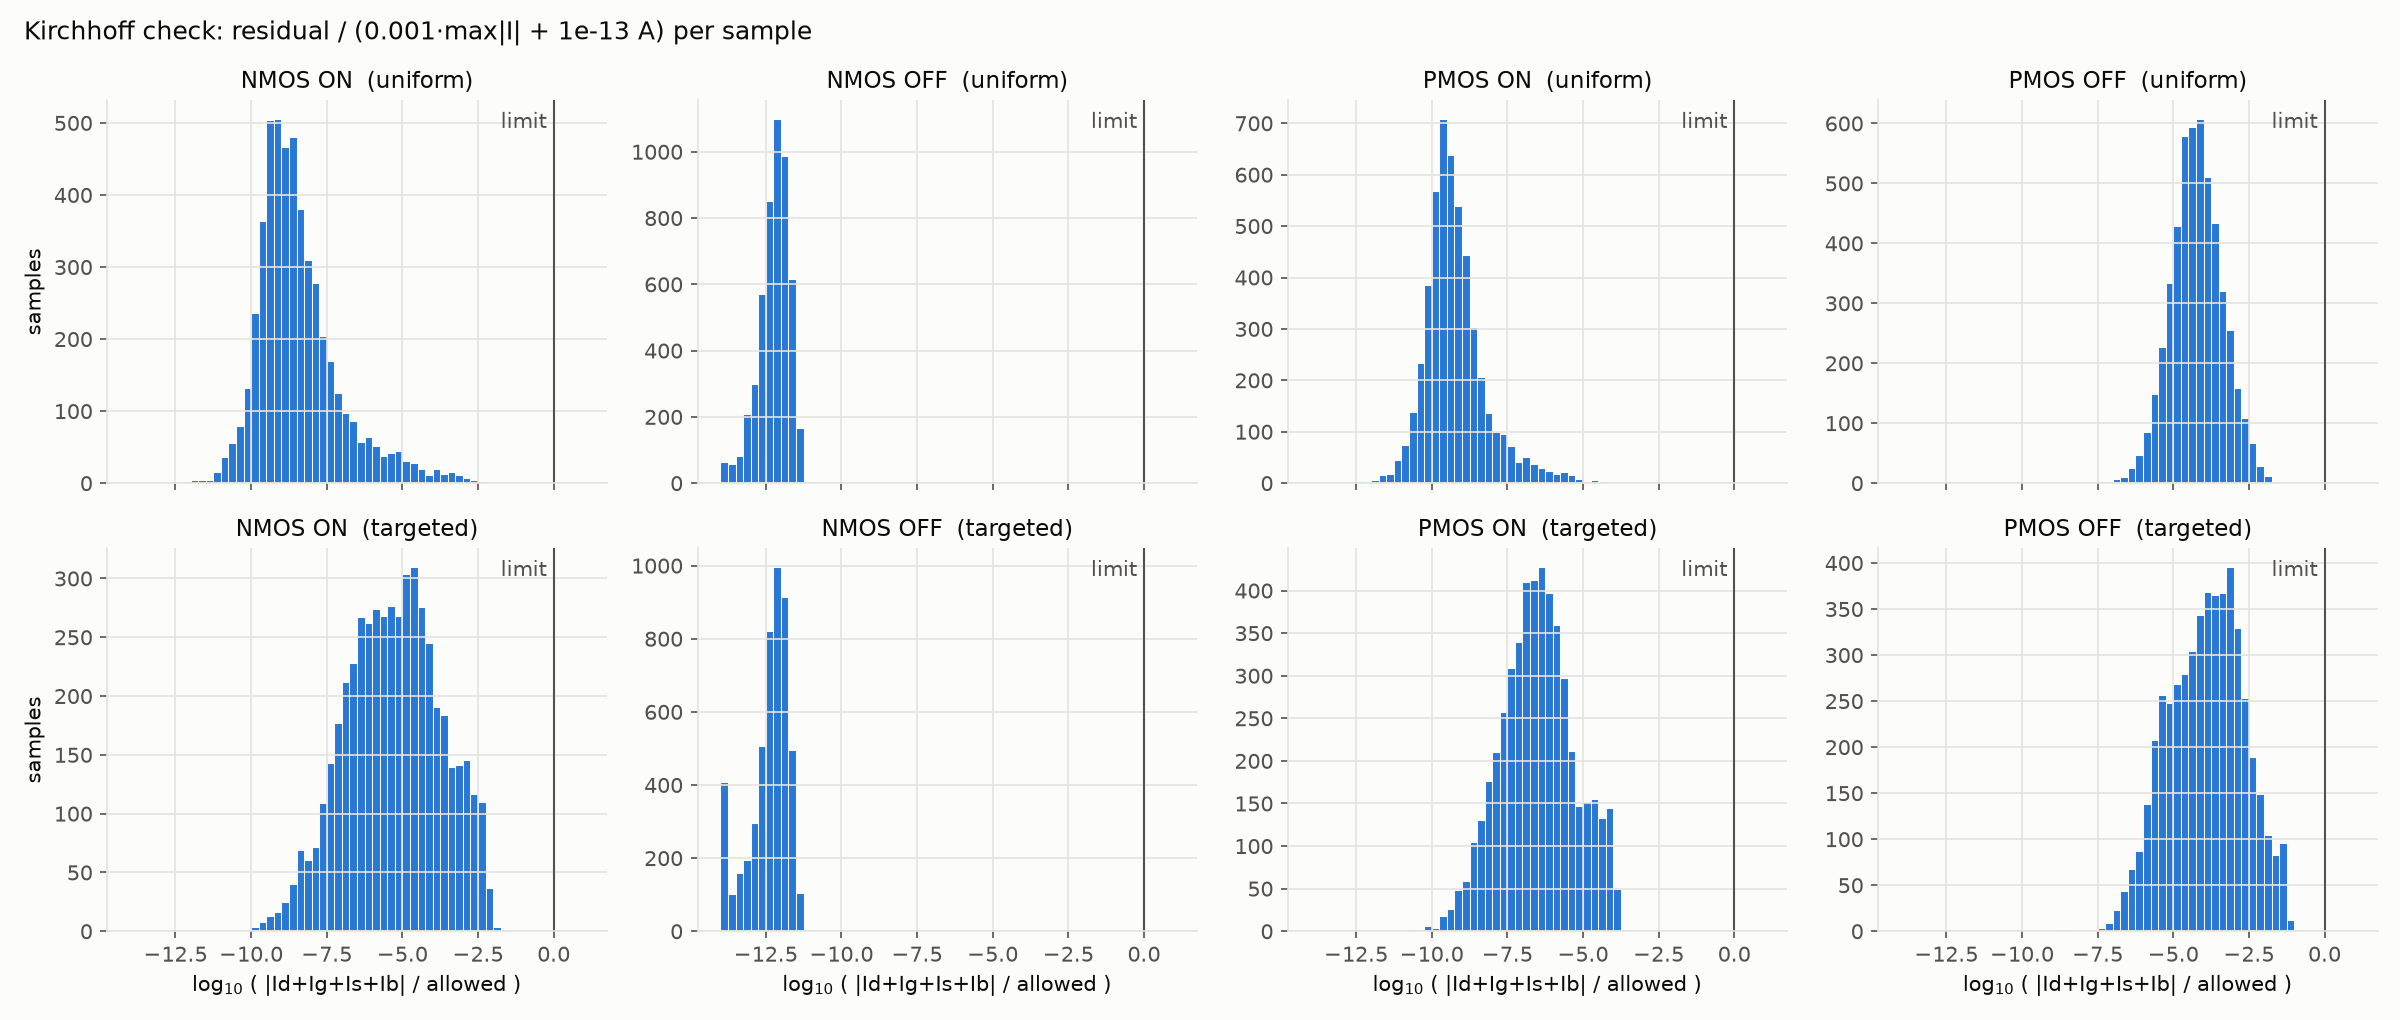
\includegraphics[width=0.6\textwidth]{kcl_check.png}
\caption{Sum of the four terminal currents for every row.}
\label{fig:kcl}
\end{figure}

\begin{figure}[H]
\centering
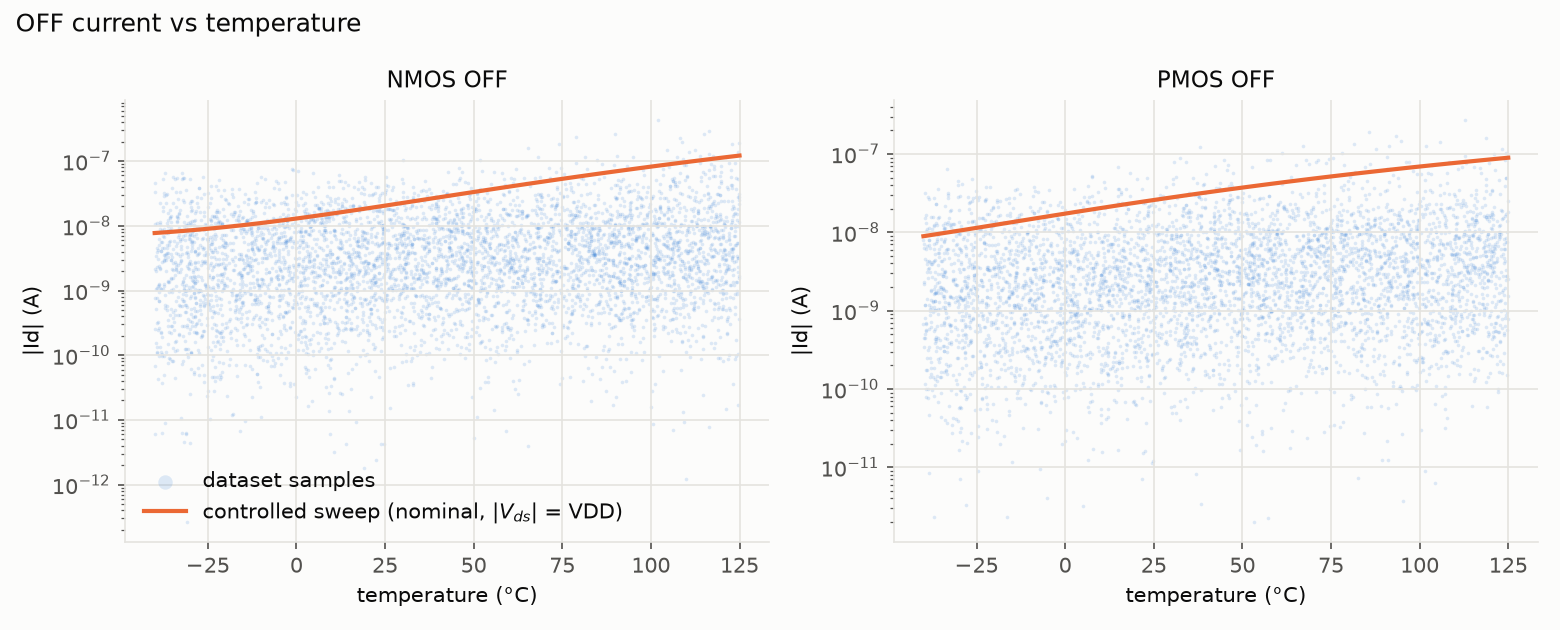
\includegraphics[width=0.6\textwidth]{off_current_vs_temp.png}
\caption{OFF current vs temperature.}
\label{fig:temp}
\end{figure}

\begin{figure}[H]
\centering
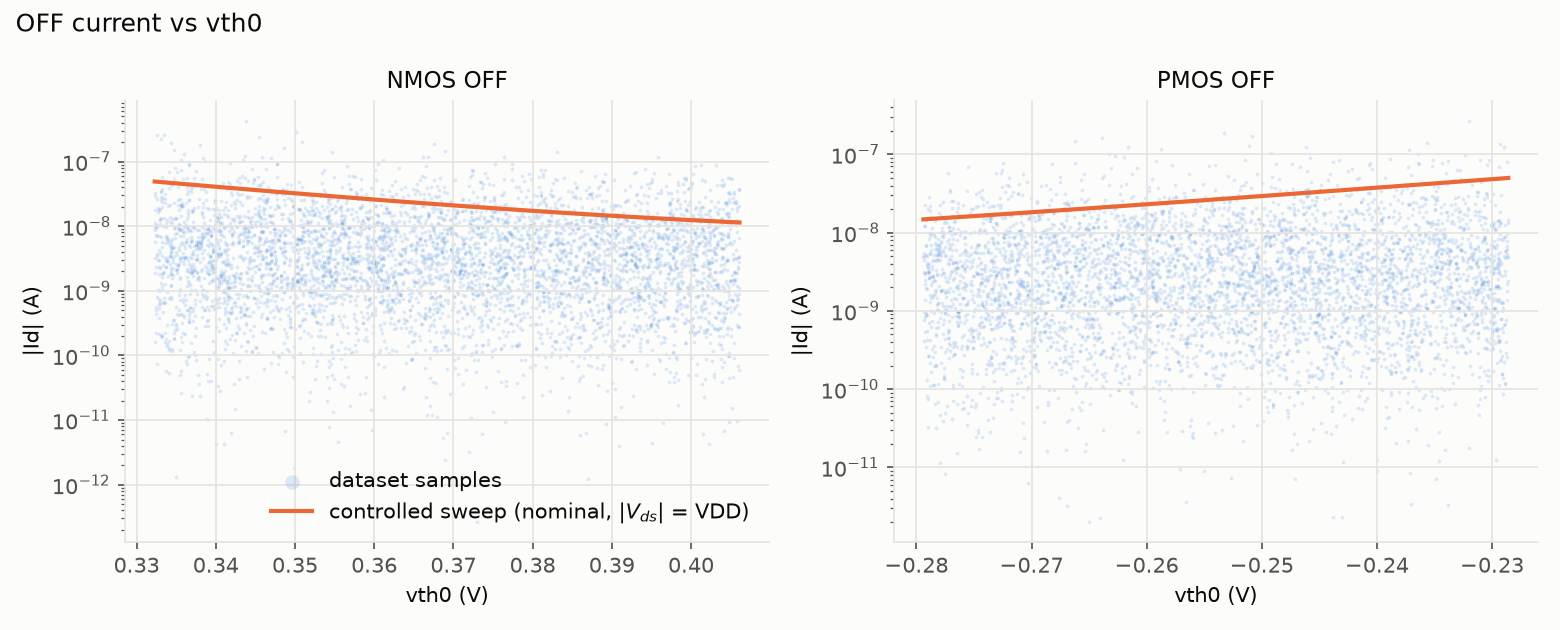
\includegraphics[width=0.6\textwidth]{off_current_vs_vth0.png}
\caption{OFF current vs vth0.}
\label{fig:vth0}
\end{figure}

\begin{figure}[H]
\centering
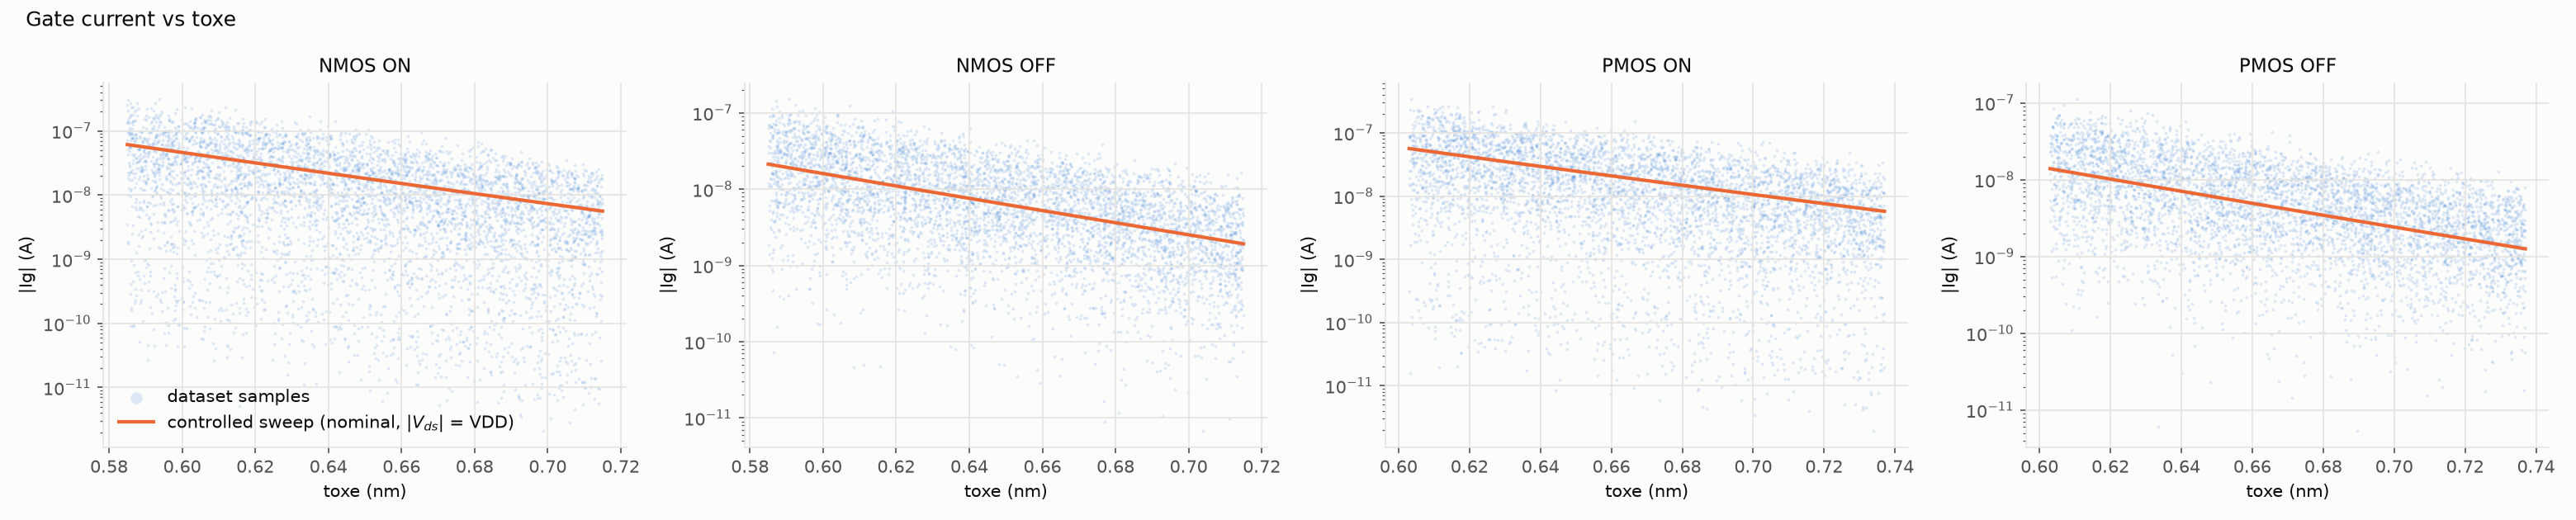
\includegraphics[width=0.9\textwidth]{gate_current_vs_toxe.png}
\caption{Gate current vs toxe.}
\label{fig:toxe}
\end{figure}

\begin{center}
{\Large\textbf{Part 2: Transistor-Level ML Models}}\\[2pt]
ML-Driven PVT-Variation-Aware Leakage Estimation \quad$\cdot$\quad Member 2: Pranav Adarsh
\end{center}

\section*{Data and method}
Each of the four transistor cases (NMOS/PMOS, ON/OFF; 22\,nm MGK, ngspice, junction areas
$AD=AS=W\times2L_\mathrm{min}$) has 10,000 SPICE rows: 5,000 with $V_\mathrm{d}, V_\mathrm{s}$ uniform
in $[0,V_\mathrm{DD}]$ and 5,000 targeted at the voltages transistors see inside gates. The 12 inputs
($V_\mathrm{DD}$, temperature, $W$, terminal voltages, vth0, toxe, ndep, u0, xj) predict
$I_\mathrm{d}, I_\mathrm{g}, I_\mathrm{s}, I_\mathrm{b}$. Data is split 70/15/15 with a fixed seed (42).

Because currents span 15 decades, each model predicts $y=\log_{10}|I|$ and a LightGBM classifier
predicts the sign, so $I=\operatorname{sign}(I)\cdot10^{y}$. The inputs are extended with
physics-based features: voltage differences, $1/kT$, log process parameters and subthreshold
exponents such as $(V_\mathrm{gs}-|\mathrm{vth0}|)/kT$.

\section*{Models and selection}
The four families were chosen to span the main kinds of regression model, from a simple baseline
to a flexible neural network, so the comparison shows how much model complexity the leakage
problem needs:
\begin{itemize}
  \item \textbf{Polynomial ridge} (degree 2--3): the baseline. It is fast and interpretable and
        tests whether a smooth fixed functional form of the physics features is enough.
  \item \textbf{Random forest} (400 trees): a robust, widely used non-linear model that needs no
        feature scaling and little tuning, giving a reference for tree-based methods.
  \item \textbf{LightGBM} (boosted trees, early stopping): usually the most accurate model on
        tabular data such as SPICE sweeps, and fast to train.
  \item \textbf{MLP} (3$\times$64 tanh, L-BFGS): a smooth function approximator suited to the
        continuous, exponential device equations; one network predicts all four currents, so they
        share what it learns about the device.
\end{itemize}
For each case the model with the lowest validation score, mean over terminals of
$(\text{median}+\text{p95})/2$ relative error, was chosen.

\begin{table}[H]
\centering\small
\begin{tabular}{lcccc|cc}
\toprule
 & \multicolumn{4}{c|}{Validation median / p95 error (\%)} & \multicolumn{2}{c}{Test median / p95 (\%)} \\
Case & Poly ridge & Rand.\ forest & LightGBM & MLP & uniform & targeted \\
\midrule
NMOS ON  & 14.0 / 74 & 13.3 / 68 & 5.8 / 31 & \textbf{2.8 / 29} & 2.1 / 8  & 4.5 / 51 \\
NMOS OFF & 19.4 / 99 & 9.1 / 51  & 5.5 / 33 & \textbf{2.8 / 12} & 2.6 / 11 & 3.5 / 15 \\
PMOS ON  & 12.4 / 67 & 12.9 / 61 & \textbf{5.4 / 30} & 2.5 / 37 & 5.0 / 21 & 6.7 / 40 \\
PMOS OFF & 21.0 / 94 & 9.9 / 52  & 5.5 / 31 & \textbf{2.9 / 13} & 2.6 / 13 & 3.3 / 14 \\
\bottomrule
\end{tabular}
\caption{Model comparison (mean of four terminals). Bold: chosen model; test columns are for the
chosen model.}
\label{tab:results}
\end{table}

\section*{Results}
The MLP had the lowest median error in every case and was chosen for NMOS ON, NMOS OFF and PMOS OFF.
For PMOS ON, LightGBM won on the selection score (17.6 vs 19.7) through its better p95, although
the MLP's median is lower; the rule's choice was kept (using the MLP changes gate accuracy by under
0.1 point). On the test sets the chosen models reach 2.1--2.6\% median error on typical points
(5.0\% for PMOS ON), with $R^2 \ge 0.98$ on $\log_{10}|I|$ and the correct sign in 98--100\% of rows
(Table~\ref{tab:results}). The largest errors are the OFF body current (junction leakage) and the
ON-device $I_\mathrm{d}, I_\mathrm{s}$ at $V_\mathrm{ds}\approx0$, which the gate formula does not use.

Used in Parts 3 and 4, the models give \textbf{1.33\% median error (98.2\% mean accuracy)} over
3,600 gate simulations and \textbf{1.14\% median (98.6\% mean accuracy)} over 102,400 simulations of
the 9-input parity checker. The learning curve shows the OFF and PMOS ON models still improving at
7k training rows, so more targeted data or an MLP ensemble could close the gap to 99\%.

\begin{figure}[H]
\centering
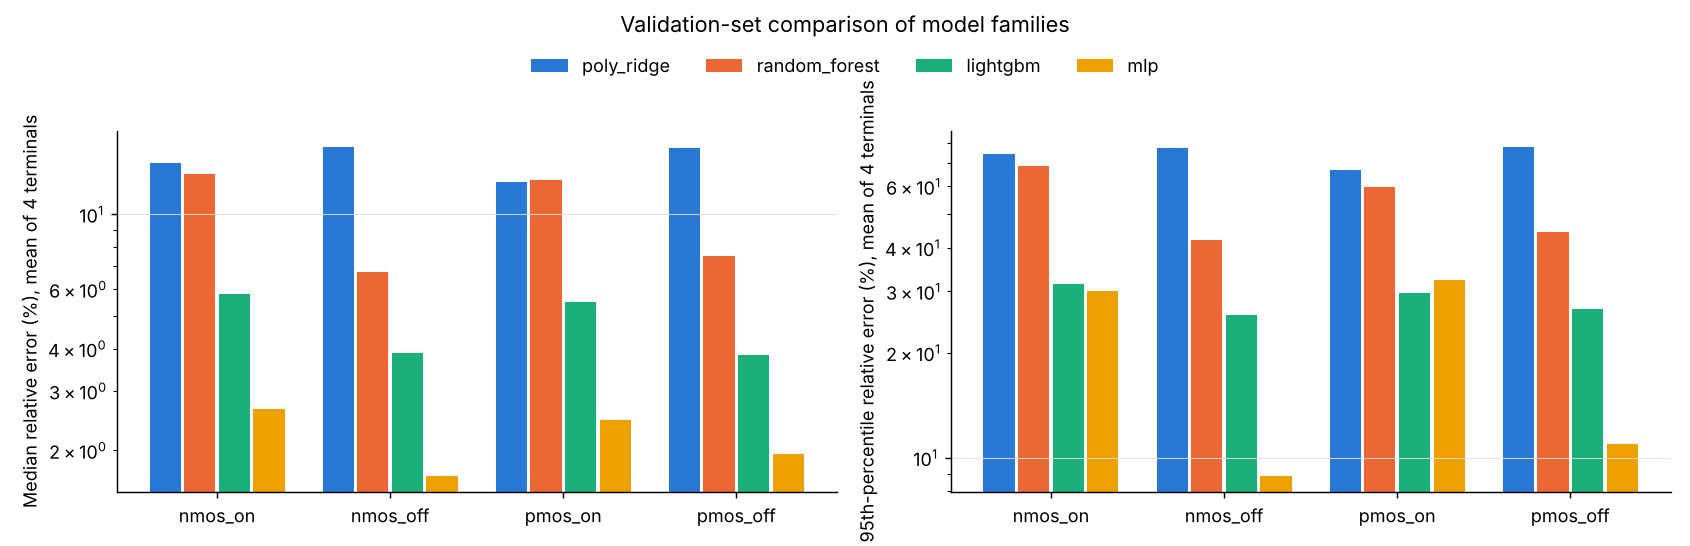
\includegraphics[width=\linewidth]{family_comparison.png}
\caption{Validation error of the four model families per case: median (left) and p95 (right).}
\end{figure}

\begin{figure}[H]
\centering
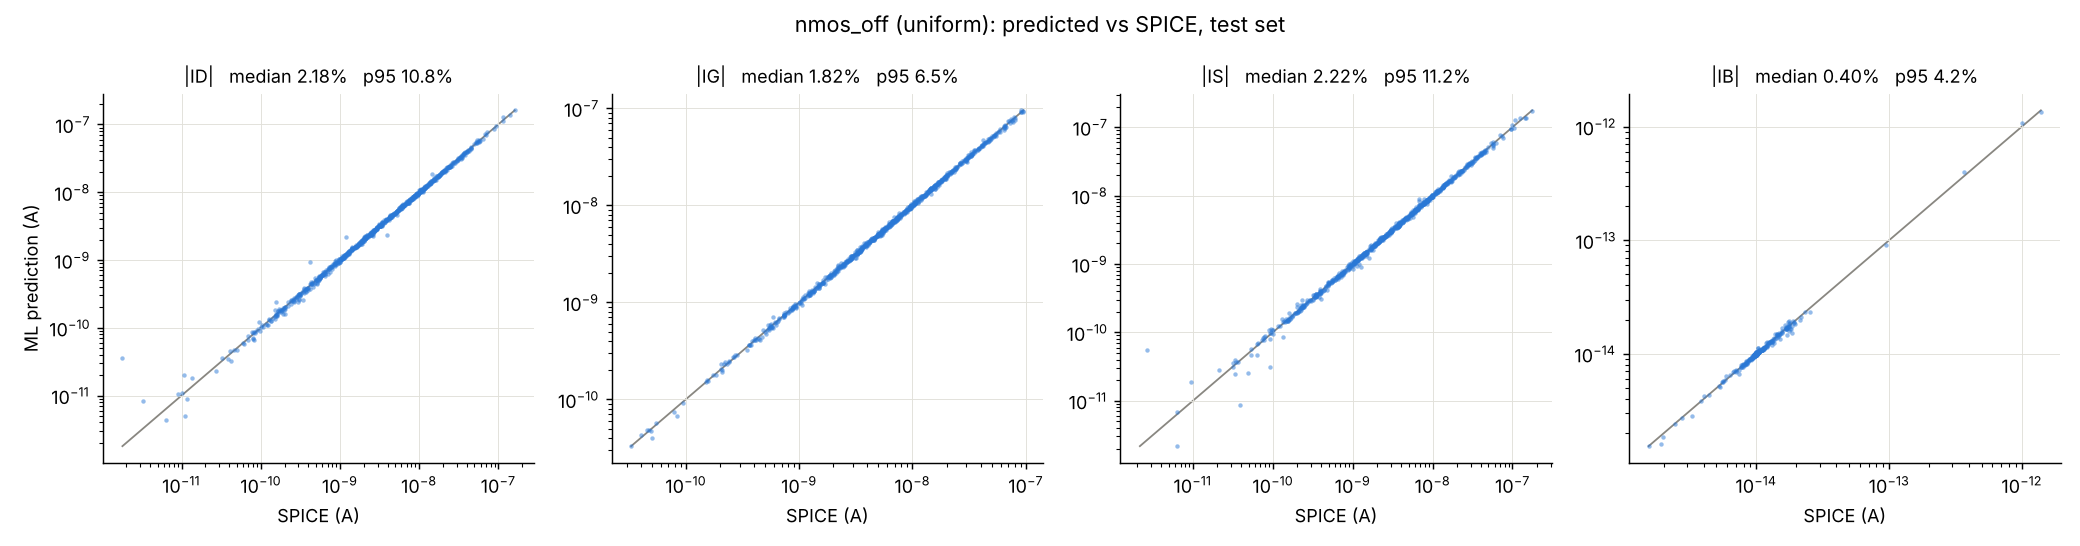
\includegraphics[width=\linewidth]{parity_nmos_off.png}
\caption{Predicted vs SPICE currents, NMOS OFF, uniform test set.}
\end{figure}

\begin{figure}[H]
\centering
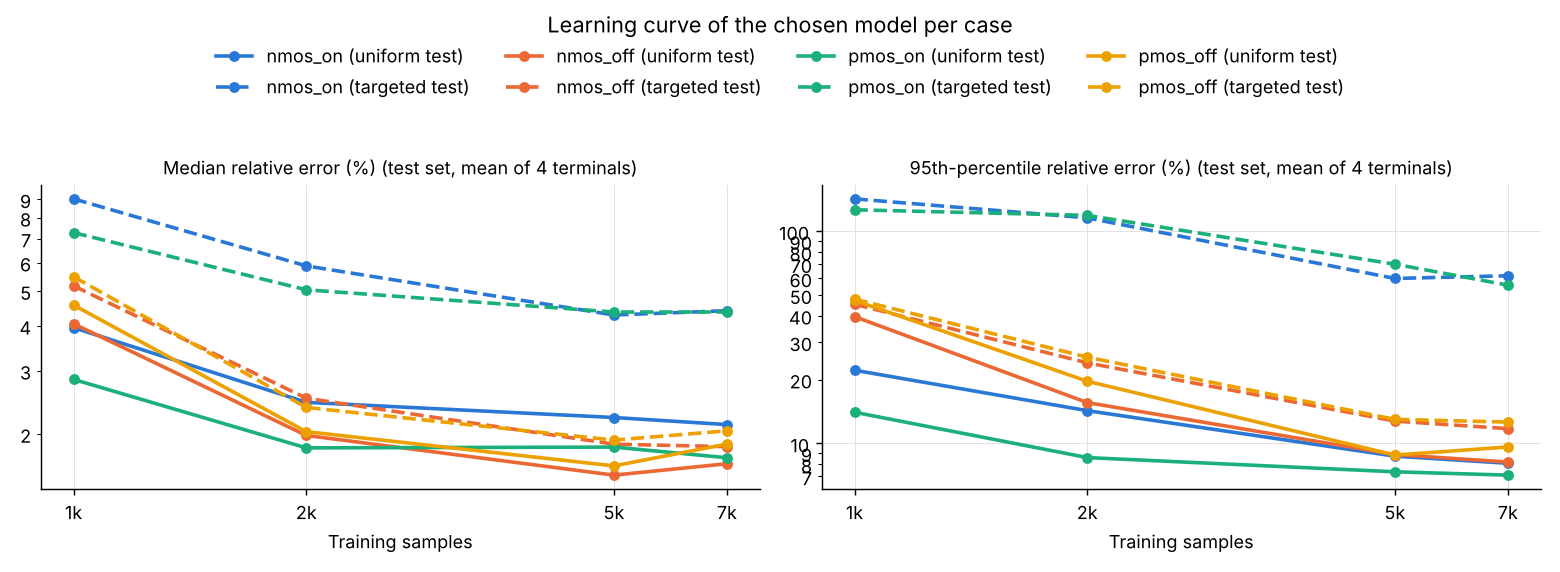
\includegraphics[width=\linewidth]{learning_curve.png}
\caption{Learning curve of the chosen model per case (solid: uniform test; dashed: targeted test).}
\end{figure}

\begin{figure}[H]
\centering
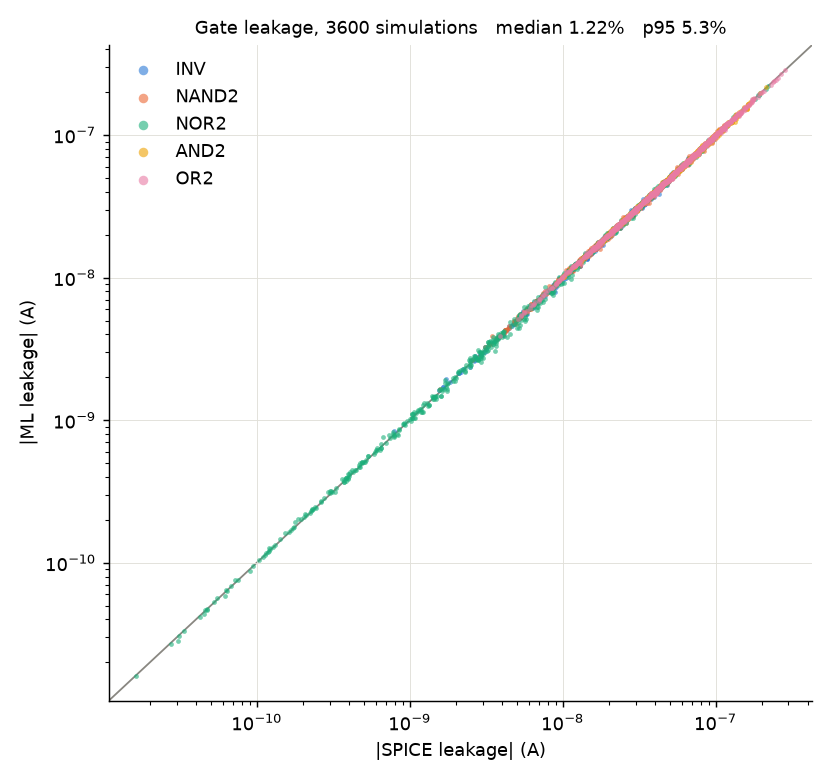
\includegraphics[width=0.55\linewidth]{gate_parity.png}
\caption{Gate leakage, ML vs SPICE, over all 3,600 gate simulations.}
\end{figure}




%%my part - Abhinav 
\section{Gate-Level Validation}

\subsection{Aim}

The transistor models predict the currents of a single transistor. This part
checks whether they can also predict the leakage of a complete logic gate.
\begin{itemize}
    \item \textbf{Leakage of a gate:} the DC current it draws from the
          $V_{DD}$ supply while its inputs are held at 0 or $V_{DD}$.
    \item \textbf{Method:} find the leakage with SPICE and with the models,
          then compare the two.
\end{itemize}

\subsection{Gates tested}

We used five static CMOS gates. Every transistor is minimum size,
$W = L = 22$\,nm.

\begin{table}[H]
\centering
\begin{tabular}{|l|l|l|c|}
\hline
Gate & Transistors & Internal nodes & Input cases \\
\hline
INV   & 1 PMOS, 1 NMOS                   & none                 & 2 \\
NAND2 & 2 parallel PMOS, 2 series NMOS   & $x$, between the two NMOS & 4 \\
NOR2  & 2 series PMOS, 2 parallel NMOS   & $y$, between the two PMOS & 4 \\
AND2  & NAND2 followed by INV            & $x$ and the NAND2 output  & 4 \\
OR2   & NOR2 followed by INV             & $y$ and the NOR2 output   & 4 \\
\hline
\end{tabular}
\caption{Gates used for the validation: 18 input cases in total.}
\label{tab:gates}
\end{table}

\begin{itemize}
    \item Inputs are written $A$ then $B$: NAND2 \texttt{01} means $A = 0$,
          $B = V_{DD}$.
    \item NAND2 stack: the NMOS driven by $A$ is next to the output, the one
          driven by $B$ is next to ground.
    \item NOR2 stack: the PMOS driven by $A$ is next to $V_{DD}$, the one
          driven by $B$ is next to the output.
\end{itemize}

\subsection{PVT corners}

A corner is one operating condition. We drew 200 corners at random, from the
same ranges as the datasets.

\begin{table}[H]
\centering
\begin{tabular}{|l|l|}
\hline
Part of a corner & Range \\
\hline
Supply voltage $V_{DD}$ & 0.81 to 0.99\,V \\
Temperature & $-40$ to $125\,^\circ$C \\
vth0, toxe, ndep, u0, xj for all NMOS & nominal $\pm 10\%$ \\
vth0, toxe, ndep, u0, xj for all PMOS & nominal $\pm 10\%$ \\
\hline
\end{tabular}
\caption{Contents of one PVT corner.}
\label{tab:corner}
\end{table}

The same 200 corners are used for every gate, and again for the parity
checker. In total there are $18 \times 200 = 3600$ simulations.

\subsection{SPICE reference}

For every case and corner, a Python script writes a netlist and runs an
\texttt{.op} (DC operating point) analysis in ngspice. The lines below are
from the NAND2 netlist with $A = B = 1$ at corner 0. They show the sources
and the first transistor; the other three transistors are written the same
way.

Each transistor terminal is connected to its node through a 0\,V source.
This does not change the circuit, but SPICE reports the current through it.
Each simulation therefore records:
\begin{itemize}
    \item the current delivered by \texttt{vsupply}, which is the reference
          leakage;
    \item the four terminal currents of every transistor;
    \item the voltages of the output and the internal nodes.
\end{itemize}

\subsection{Leakage from the models}

The estimate is made in three steps for each simulation.
\begin{enumerate}
    \item \textbf{Terminal voltages.} Inputs are 0 or $V_{DD}$. The output
          and internal node voltages are taken from the SPICE run, because
          the models predict currents and not voltages.
    \item \textbf{Terminal currents.} A transistor is ON if its gate voltage
          is above $V_{DD}/2$ (NMOS) or below it (PMOS). The model for its
          case predicts $I_d$, $I_g$, $I_s$ and $I_b$.
    \item \textbf{Supply current.} The predicted currents are combined into
          the current drawn from $V_{DD}$ (Section~\ref{sec:combine}).
\end{enumerate}

\subsection{Combining the currents}
\label{sec:combine}

The project statement says to use the predicted currents to calculate the
gate leakage, but it does not give a formula. We used two methods. Both use
only the currents predicted by the models.

\paragraph{Method 1: direct sum.}
The supply current is the sum of the currents into all transistor terminals
connected to $V_{DD}$:
\begin{equation}
I_{VDD} = \sum_{\mathrm{terminals\ at\ } V_{DD}} I_{\mathrm{terminal}}.
\end{equation}
This is the simplest method, but it has a weak point:
\begin{itemize}
    \item the sum contains the source current of every ON PMOS connected to
          $V_{DD}$;
    \item an ON transistor inside a gate has almost no voltage across it, so
          its channel carries only what the OFF transistors let through;
    \item the models predict this small current poorly.
\end{itemize}

\paragraph{Method 2: KCL formula (main result).}
The same sum is used, but the drain and source currents of ON transistors
are never taken from the models. They are replaced using KCL: the currents
into a node add up to zero, and so do the four currents of one transistor.

\begin{table}[H]
\centering
\begin{tabular}{|l|l|l|}
\hline
Transistor & Method 1 uses & Method 2 uses \\
\hline
OFF & $I_d$, $I_g$, $I_s$, $I_b$ & $I_d$, $I_g$, $I_s$, $I_b$ \\
ON  & $I_d$, $I_g$, $I_s$, $I_b$ & $I_g$ and $I_b$ only; channel current from KCL \\
\hline
\end{tabular}
\caption{Predicted currents used by the two methods.}
\label{tab:used}
\end{table}

With exact currents the two methods give the same answer. They differ only
because the predicted currents have errors.

\subsection{Example: inverter with input 0}

The PMOS is ON and the NMOS is OFF. The source and body of the PMOS are
connected to $V_{DD}$.

\paragraph{Method 1.}
\begin{equation}
I_{VDD} = I_s^{P} + I_b^{P}.
\end{equation}
This uses the source current of the ON PMOS.

\paragraph{Method 2.}
KCL for the PMOS, and KCL at the output node, give
\begin{equation}
I_s^{P} = -\left(I_d^{P} + I_g^{P} + I_b^{P}\right), \qquad
I_d^{P} + I_d^{N} = 0.
\end{equation}
Putting these into the Method 1 sum:
\begin{equation}
I_{VDD} = I_d^{N} - I_g^{P}.
\end{equation}
The leakage is the drain current of the OFF NMOS plus the gate current
leaving the ON PMOS. The source current of the ON PMOS is no longer needed.
The other gates are handled the same way, with one KCL equation per internal
node.

\subsection{Check of the formulas}

Before using the models, the terminal currents recorded by SPICE were put
through both methods and compared with the supply current from SPICE, in all
3600 simulations.
\begin{itemize}
    \item Method 1 matches within a relative difference of $10^{-15}$.
    \item Method 2 matches within $4.5 \times 10^{-7}$.
    \item Both formulas are therefore correct, and the errors reported below
          come from the models.
\end{itemize}

\subsection{Results}

All results in this section use Method 2. The error of one simulation is
$|I_{ML} - I_{SPICE}| / |I_{SPICE}|$. The bias is the median of
$(I_{ML} - I_{SPICE}) / I_{SPICE}$, so a negative bias means the estimate is
usually too low. Table~\ref{tab:gateoverall} gives the error over all 3600 simulations,
Fig.~\ref{fig:gateparity} shows every simulation, and
Table~\ref{tab:gateresults} gives the error of each case.

\begin{table}[H]
\centering
\begin{tabular}{|l|r|}
\hline
Median error & 1.30\% \\
95th percentile (p95) error & 4.78\% \\
Mean error & 1.76\% (98.2\% mean accuracy) \\
Simulations with error below 5\% & 95.5\% \\
Simulations with error below 10\% & 99.7\% \\
\hline
\end{tabular}
\caption{Error of the gate leakage over all 3600 simulations.}
\label{tab:gateoverall}
\end{table}

\begin{figure}[H]
\centering
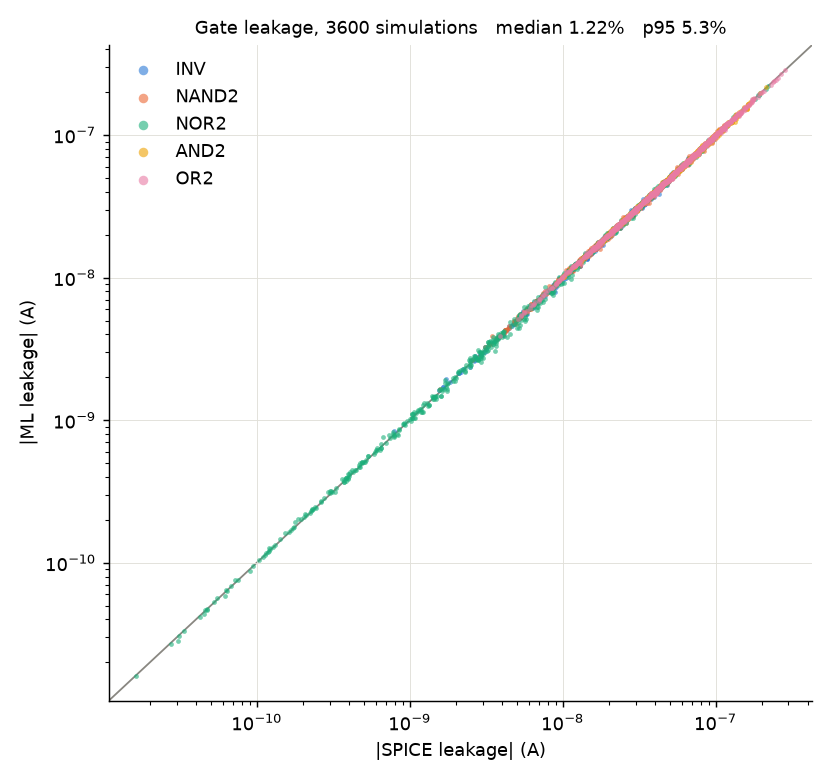
\includegraphics[width=0.4\textwidth]{gate_parity.png}
\caption{Gate leakage from the models against gate leakage from SPICE for
all 3600 simulations. Points on the diagonal line are exact.}
\label{fig:gateparity}
\end{figure}

\begin{table}[H]
\centering
\begin{tabular}{|l|c|r|r|r|r|r|r|}
\hline
     &        & \multicolumn{2}{c|}{Median leakage (nA)} & & \multicolumn{3}{c|}{Error} \\
\cline{3-4}\cline{6-8}
Gate & Inputs & SPICE & ML & Bias & Median & p95 & Mean \\
\hline
INV   & 0  & 25.40 & 25.78 & $-0.31\%$ & 1.30\% & 3.63\% & 1.49\% \\
INV   & 1  & 14.53 & 14.48 & $+0.12\%$ & 1.60\% & 5.32\% & 1.98\% \\
\hline
NAND2 & 00 & 20.55 & 20.53 & $+0.17\%$ & 1.40\% & 4.96\% & 1.81\% \\
NAND2 & 01 & 25.33 & 25.69 & $-0.38\%$ & 1.33\% & 3.65\% & 1.48\% \\
NAND2 & 10 & 18.93 & 18.82 & $-0.18\%$ & 1.23\% & 3.55\% & 1.41\% \\
NAND2 & 11 & 29.00 & 28.90 & $+0.11\%$ & 1.60\% & 5.34\% & 1.97\% \\
\hline
NOR2  & 00 & 50.51 & 51.17 & $-0.36\%$ & 1.33\% & 3.56\% & 1.51\% \\
NOR2  & 01 & 24.80 & 24.73 & $-0.06\%$ & 1.19\% & 4.08\% & 1.44\% \\
NOR2  & 10 & 8.57  & 8.17  & $-3.38\%$ & 3.88\% & 8.06\% & 3.93\% \\
NOR2  & 11 & 0.74  & 0.74  & $-1.08\%$ & 3.29\% & 8.97\% & 4.49\% \\
\hline
AND2  & 00 & 51.29 & 50.96 & $+0.04\%$ & 0.99\% & 3.23\% & 1.23\% \\
AND2  & 01 & 56.16 & 55.72 & $-0.18\%$ & 0.88\% & 2.86\% & 1.13\% \\
AND2  & 10 & 48.16 & 47.70 & $-0.07\%$ & 0.84\% & 2.89\% & 1.03\% \\
AND2  & 11 & 58.16 & 57.19 & $-0.19\%$ & 1.11\% & 3.16\% & 1.31\% \\
\hline
OR2   & 00 & 83.11 & 83.52 & $-0.36\%$ & 0.98\% & 3.02\% & 1.19\% \\
OR2   & 01 & 54.39 & 54.05 & $-0.29\%$ & 0.95\% & 3.29\% & 1.22\% \\
OR2   & 10 & 35.53 & 35.34 & $-1.30\%$ & 1.59\% & 3.57\% & 1.64\% \\
OR2   & 11 & 26.99 & 27.36 & $-0.39\%$ & 1.23\% & 3.52\% & 1.45\% \\
\hline
All   &    & 30.25 & 30.28 & $-0.32\%$ & 1.30\% & 4.78\% & 1.76\% \\
\hline
\end{tabular}
\caption{Gate results for each case (Method 2). Each row covers the 200
corners.}
\label{tab:gateresults}
\end{table}

\subsection{Where the error is largest and smallest}

\paragraph{Largest: NOR2 \texttt{10} and \texttt{11} (3.9\% and 3.3\% median).}
\begin{itemize}
    \item The PMOS next to $V_{DD}$ is OFF, and its source current is more
          than 99.99\% of the supply current. The estimate depends on this
          one predicted current.
    \item Its drain is at the internal node $y$: 0.15 to 0.20\,$V_{DD}$ in
          case \texttt{10}, and 0.89 to 0.93\,$V_{DD}$ in case \texttt{11}.
    \item Only about 35 of the 10{,}000 PMOS OFF training rows lie in each
          of these regions, so the model is less accurate there.
\end{itemize}

\paragraph{Smallest: AND2 and OR2 (1.0\% and 1.2\% median).}
Their leakage is the sum of two stages, so it does not depend on a single
predicted current.

\subsection{One estimate with the wrong sign}

\begin{table}[H]
\centering
\begin{tabular}{|l|l|}
\hline
Simulation & NOR2 \texttt{11}, corner 76 ($-38\,^\circ$C) \\
SPICE leakage & $+16$\,pA, the smallest of all 3600 simulations \\
Model estimate & $-13$\,pA \\
Absolute error & 29\,pA \\
\hline
\end{tabular}
\caption{The only simulation where the estimate has the wrong sign.}
\label{tab:sign}
\end{table}

Here the source current of the OFF PMOS is the difference of a channel
current (33\,pA) and a gate current (17\,pA) that almost cancel. In the
other 3599 simulations the largest error is 14.7\%.

\subsection{Comparison of the methods}

Table~\ref{tab:variants} gives the error over all 3600 simulations for every
way of computing the leakage that we used.

\begin{table}[H]
\centering
\begin{tabular}{|l|r|r|}
\hline
Method & Median error & p95 error \\
\hline
Method 1: direct sum & 4.02\% & 15.7\% \\
Method 2: KCL formula (main result) & 1.30\% & 4.78\% \\
Method 2, inverter gate voltage set to exactly 0 or $V_{DD}$ & 1.38\% & 5.0\% \\
Method 2, also counting current from inputs at $V_{DD}$ & 1.13\% & 3.6\% \\
\hline
\end{tabular}
\caption{Error for each way of computing the gate leakage.}
\label{tab:variants}
\end{table}

\paragraph{Method 1 against Method 2.}
\begin{itemize}
    \item In four cases (INV \texttt{1}, NAND2 \texttt{11}, NOR2 \texttt{10},
          NOR2 \texttt{11}) no ON transistor is connected to $V_{DD}$ by its
          drain or source, so the two methods give the same result.
    \item In the other 14 cases the median error is 2.7\% to 8.0\% with
          Method 1 and 0.8\% to 1.6\% with Method 2.
\end{itemize}

\paragraph{Inverter gate voltage.}
\begin{itemize}
    \item In AND2 and OR2 the inverter is driven by the NAND2 or NOR2
          output, which is up to 1.8\% of $V_{DD}$ away from 0 or $V_{DD}$.
    \item The main result uses this recorded voltage. Setting it to exactly
          0 or $V_{DD}$ gives a slightly higher error.
\end{itemize}

\paragraph{Current from the inputs.}
\begin{itemize}
    \item An input held at $V_{DD}$ also supplies a small gate current. The
          main result counts only the current from the supply.
    \item In the last row this input current is counted as leakage in both
          SPICE and the estimate.
\end{itemize}

% Srikar's section. Insert immediately before \end{document}.
% Numerical results remain blank pending consistent upstream regeneration.
\clearpage
\section{Circuit-Level Validation: Parity Checker}
\label{sec:circuit}

\subsection{Aim}
This part extends the gate-level method to a complete circuit. The aim is
to estimate its static supply leakage by combining predictions for its
individual gates, and compare the estimate with a transistor-level SPICE
simulation of the complete circuit.

\subsection{Circuit construction}
The circuit checks eight data bits, $d_0,\ldots,d_7$, together with an
even-parity bit $p$. Its output is
\begin{equation}
e=d_0\oplus d_1\oplus\cdots\oplus d_7\oplus p.
\end{equation}
An output of 0 indicates valid even parity; an output of 1 indicates a
parity error. There are nine primary inputs and $2^9=512$ input vectors.
The vector order used throughout is $d_0,d_1,\ldots,d_7,p$.

The eight data bits are combined using a balanced XOR tree. Its output is
then XORed with the parity bit. Each of the eight XOR operations is built
from four NAND2 gates:
\begin{align}
t_1&=\operatorname{NAND}(a,b), &
t_2&=\operatorname{NAND}(a,t_1),\\
t_3&=\operatorname{NAND}(b,t_1), &
a\oplus b&=\operatorname{NAND}(t_2,t_3).
\end{align}
The complete circuit therefore contains 32 NAND2 gates and 128 transistors.
Each NAND2 uses the same topology and minimum transistor sizing as Part 3:
$W=L=22$\,nm. The intended consistent device setup uses drain and source
areas $AD=AS=W(2L)$. The transistor netlist contains no ideal logic gates
and no added output load.

One ordered list of gate connections is used for both Boolean evaluation
and netlist generation. NAND inputs retain their order: input $a$ drives
the upper NMOS in the stack and input $b$ drives the lower NMOS. This matters
because states \texttt{01} and \texttt{10} need not have the same leakage.

\subsection{PVT conditions and SPICE reference}
The evaluation uses the same 200 PVT corners as Part 3. Each corner specifies
the supply voltage, temperature, and separate NMOS and PMOS process
parameters. Evaluating every input vector at every corner gives
$512\times200=102{,}400$ circuit cases. These are 200 distinct PVT draws,
each reused for all 512 vectors.

The reference leakage is the current drawn from the complete circuit's
shared supply, $I_{\mathrm{SPICE}}=-i(\texttt{vsupply})$. Current supplied by
the separate primary-input sources is excluded from this main definition.
The simulator records the supply current, primary-input currents, and all
32 NAND output voltages. A DC sweep enumerates the binary inputs using
sources that hold each input at exactly 0 or $V_{DD}$. The circuit itself
remains a transistor-level circuit. Independent operating-point simulations
provide a cross-check of this sweep method.

\subsection{Hierarchical estimate from the transistor models}
The circuit estimate reuses the Part 3 NAND2 predictions. At each corner,
a lookup table contains the four ordered NAND input states, giving
$4\times200=800$ entries. Each entry contains the gate's predicted supply
leakage and the signed gate currents at its two input pins. The supply
leakage uses the KCL method described in Section~\ref{sec:combine}.
For a NAND input pin, its current is the sum of the gate-terminal currents
of the PMOS and NMOS connected to that pin.

For each nine-bit input vector, Boolean evaluation determines the input
state of every NAND. The corresponding lookup entry is selected for each
gate and the contributions are combined. The circuit estimate does not
use node voltages from the complete-circuit SPICE simulation. However,
the isolated-gate lookup inherits the SPICE-recorded transistor voltages
used by Part 3; it is therefore a hierarchical approximation based on
characterised gates.

\subsection{Combining the gate contributions}
\paragraph{Plain gate sum (baseline).}
The prescribed hierarchical estimate adds the supply leakages of the
32 isolated NAND gates:
\begin{equation}
\widehat I_{\mathrm{plain}}=\sum_{j=1}^{32}\widehat I_{\mathrm{supply},j}.
\end{equation}
This baseline is retained in the comparison.

\paragraph{Correction for internally driven high inputs.}
An isolated gate's input is powered by an external voltage source. Inside
the circuit, an internal high input is instead driven by another gate,
which must supply its input gate current. The plain sum omits this
contribution. Under the ideal-rail approximation, the corrected estimate is
\begin{equation}
\widehat I_{\mathrm{corrected}}=
\widehat I_{\mathrm{plain}}+
\sum_{(j,q)\in\mathcal H_{\mathrm{internal}}}\widehat I_{g,jq},
\end{equation}
where $\mathcal H_{\mathrm{internal}}$ contains the receiving input pins
that are high and driven by another gate. Currents are signed, positive
into the receiving pin; their absolute values are not used. Each receiving
pin is counted once, including when a driver has multiple loads.

Primary-input currents remain excluded because their sources are separate
from the circuit supply. A separate variant adds the currents at high
primary inputs to both the prediction and the SPICE reference, so that the
two sides still use the same leakage definition. The correction changes
current accounting; it does not solve the circuit's coupled analog voltages.

\subsection{Validation procedure}
The implementation includes the following checks:
\begin{itemize}
\item Exhaustive Boolean evaluation of all 512 vectors, including checking
      that flipping the parity bit flips the error output.
\item Structural checks for an ordered, acyclic graph with 32 NAND2 gates
      and a generated netlist containing 128 transistors.
\item Checks of every simulated NAND output against its Boolean value,
      primary-input voltages against their required rails, and complete
      coverage of the corner--vector pairs.
\item Tests of signed input-current ownership, agreement between batched
      and individual aggregation, and rejection of missing or incorrect
      simulation measurements.
\item An independent operating-point versus DC-sweep comparison.
\end{itemize}
\noindent\textit{Final validation outcomes and simulator version: pending
the run with consistently regenerated datasets and models.}

\subsection{Results}
For each circuit case, the relative error and signed relative error are
\begin{equation}
r=\frac{|\widehat I-I_{\mathrm{SPICE}}|}{|I_{\mathrm{SPICE}}|},
\qquad
b=\frac{\widehat I-I_{\mathrm{SPICE}}}{I_{\mathrm{SPICE}}}.
\end{equation}
The comparison reports median, 95th-percentile and mean relative error;
bias is the median signed relative error. Under the project's convention,
mean accuracy is $100(1-\operatorname{mean}(r))\%$.

\begin{table}[H]
\centering\small
\begin{tabular}{lrrrr}
\toprule
Estimate & Bias (\%) & Median error (\%) & p95 (\%) & Mean (\%)\\
\midrule
Plain gate sum & & & & \\
Corrected supply estimate & & & & \\
Including primary high inputs & & & & \\
\bottomrule
\end{tabular}
\caption{Circuit comparison. Numerical cells are intentionally blank pending
the final consistent run.}
\label{tab:circuitresults}
\end{table}

\begin{table}[H]
\centering
\begin{tabular}{lr}
\toprule
Quantity (supply-only comparison) & Value\\
\midrule
Median SPICE leakage ($\mu$A) & \\
Median corrected ML leakage ($\mu$A) & \\
Maximum corrected relative error (\%) & \\
Corrected mean accuracy (\%) & \\
\bottomrule
\end{tabular}
\caption{Additional circuit metrics, to be filled after the final run.}
\end{table}

\begin{figure}[H]
\centering
\fbox{\parbox[c][35mm][c]{0.85\linewidth}{\centering
Pending final circuit parity plot: plain and corrected ML estimates
against complete-circuit SPICE, with logarithmic axes.}}
\caption{Placeholder for the final circuit leakage comparison.}
\label{fig:circuitparity}
\end{figure}

\begin{figure}[H]
\centering
\fbox{\parbox[c][35mm][c]{0.85\linewidth}{\centering
Pending final plot of corrected relative error against temperature.}}
\caption{Placeholder for the final temperature-dependent error plot.}
\label{fig:circuittemperature}
\end{figure}

\subsection{Worked calculation}
For vector \texttt{000000000} at corner 0, Boolean evaluation gives eight
NAND gates in state \texttt{00}, sixteen in \texttt{01}, none in
\texttt{10}, and eight in \texttt{11}. Thus,
\begin{equation}
\widehat I_{\mathrm{plain}}=
8\widehat I_{00}+16\widehat I_{01}+8\widehat I_{11}.
\end{equation}
The internal high-input currents are then added and the result is compared
with the complete-circuit supply current.
\begin{table}[H]
\centering
\begin{tabular}{lr}
\toprule
Calculation step & Value\\
\midrule
Plain gate sum ($\mu$A) & \\
Internal high-input correction ($\mu$A) & \\
Corrected estimate ($\mu$A) & \\
Complete-circuit SPICE reference ($\mu$A) & \\
Relative error (\%) & \\
\bottomrule
\end{tabular}
\caption{Worked example; numerical values await the final run.}
\end{table}

\subsection{Error analysis and limitations}
\noindent\textit{Results-dependent discussion is pending: comparison with
gate-level accuracy, worst corners and vectors, temperature dependence,
and whether the mean-accuracy objective is reached.}

The lookup assumes ideal input rails and isolated-gate operating points.
In the complete circuit, fanout and departures from ideal high and low
voltages can change leakage. The input-current correction accounts for
internally supplied input currents but does not remove this approximation.
The transistor models also retain prediction errors.

To distinguish these effects, the same aggregation is also evaluated using
isolated-gate SPICE currents in place of ML currents. Its disagreement with
complete-circuit SPICE measures the error of composing isolated gates;
comparison with the ML estimate helps assess the additional model error.
Absolute errors from these comparisons need not add, because signed errors
can cancel.

Possible improvements include gate models conditioned on analog input
voltages and loading, a coupled node-voltage solution, and improved
transistor training coverage. Circuit evaluation cases must remain outside
the training data.

\subsection{Reproducibility}
The circuit construction, simulation, comparison and validation scripts
are provided in \texttt{part4\_circuit/}. Once the consistent upstream
artifacts are available, \texttt{python run\_all.py --part4-only} runs the
Part 4 tests, circuit simulation workflow and comparison. The separate
\texttt{part4\_circuit/cross\_check.py} script performs the independent
operating-point/DC check. Final tables, plots and validation records will
be taken from that consistent run.

\end{document}
